\documentclass{bioinfo}
\copyrightyear{2012}
\pubyear{2012}

\begin{document}
\firstpage{1}

\title[istar]{istar: Software-as-a-Service Platform for idock and igrep}
\author[Hongjian Li \textit{et~al}]{Hongjian Li\footnote{to whom correspondence should be addressed}, Kwong-Sak Leung and Man-Hon Wong}
\address{Department of Computer Science and Engineering, Chinese University of Hong Kong, Shatin, New Territories, Hong Kong, China}

\history{Received on XXXXX; revised on XXXXX; accepted on XXXXX}

\editor{Associate Editor: XXXXXXX}

\maketitle

\begin{abstract}
\section{Summary:}
We were motivated by the desire to automate large-scale protein-ligand docking using our idock and thus developed istar, a general SaaS (Software as a Service) platform. Without tedious software installation, users, especially computational chemists, can submit jobs on the fly either by browsing our web site or by programming against our RESTful API. Our HTML5- and CSS3-powered web site supports filtering and previewing ligands to dock, as well as monitoring job progress in real time, two very useful features commonly lacked in other SaaS platforms like DOCK Blaster. We developed a customized daemon from idock 1.5 and implemented two-phase docking. We deployed several high-performance workstations to run the idock daemon in the background and exploited fine-grained slice-level parallelism in phase 1. The daemon compresses result files using gzip to save server storage and network bandwidth.

\section{Availability:}
istar is free and open source under Apache License 2.0. Its C++ and JavaScript source code is available at https://github.com/HongjianLi/istar. A live demo is running at http://istar.cse.cuhk.edu.hk.

\section{Contact:} \href{hjli@cse.cuhk.edu.hk}{hjli@cse.cuhk.edu.hk}
\end{abstract}

\section{Introduction}

In 2011, we developed idock 1.0 \citep{1153}, a multithreaded virtual screening tool for flexible ligand docking. In 2012, we developed idock 1.5, further improving docking speed and accuracy, inventing new functionalities, and fixing bugs. Comprehensive benchmark showed that idock 1.5 displayed comparable success rates in terms of redocking but significantly outperformed state-of-the-art AutoDock Vina 1.1.2 \citep{595} in terms of docking speed by at least 8.69 times and at most 37.51 times across 12 diverse receptors and 3000 ligands of different molecular weight.

Having released idock, we kept receiving docking requirements from our colleagues and collaborators. They are mostly biochemists and pharmacists, outsourcing the docking research to us after discovering potential biological targets for certain diseases of therapeutic interest. All of a sudden, we had to grab the protein structure, do format conversion, define search space, set up docking parameters, and keep running idock in batch for months. Tedious enough, all the above work was done manually, resulting in very low research productivity. In order to boost efficiency and automate large-scale protein-ligand docking using our idock, we therefore developed istar, a general SaaS platform.

Figure \ref{istar:architecture} shows the architecture of istar. There are five major components: a web site, a web server, a database management system, several workstations, and a network file system. Under typical circumstance, a user browses our web site and submits a job. The web server first validates user input and then saves it into database. Several workstations run daemons in the background, fetching jobs from the database and carrying out experiments. Upon completion, they send a notification email to the user and write the result to the network file system, which is served and cached as static content. The user again browses our web site to download result.

\begin{figure}
\centerline{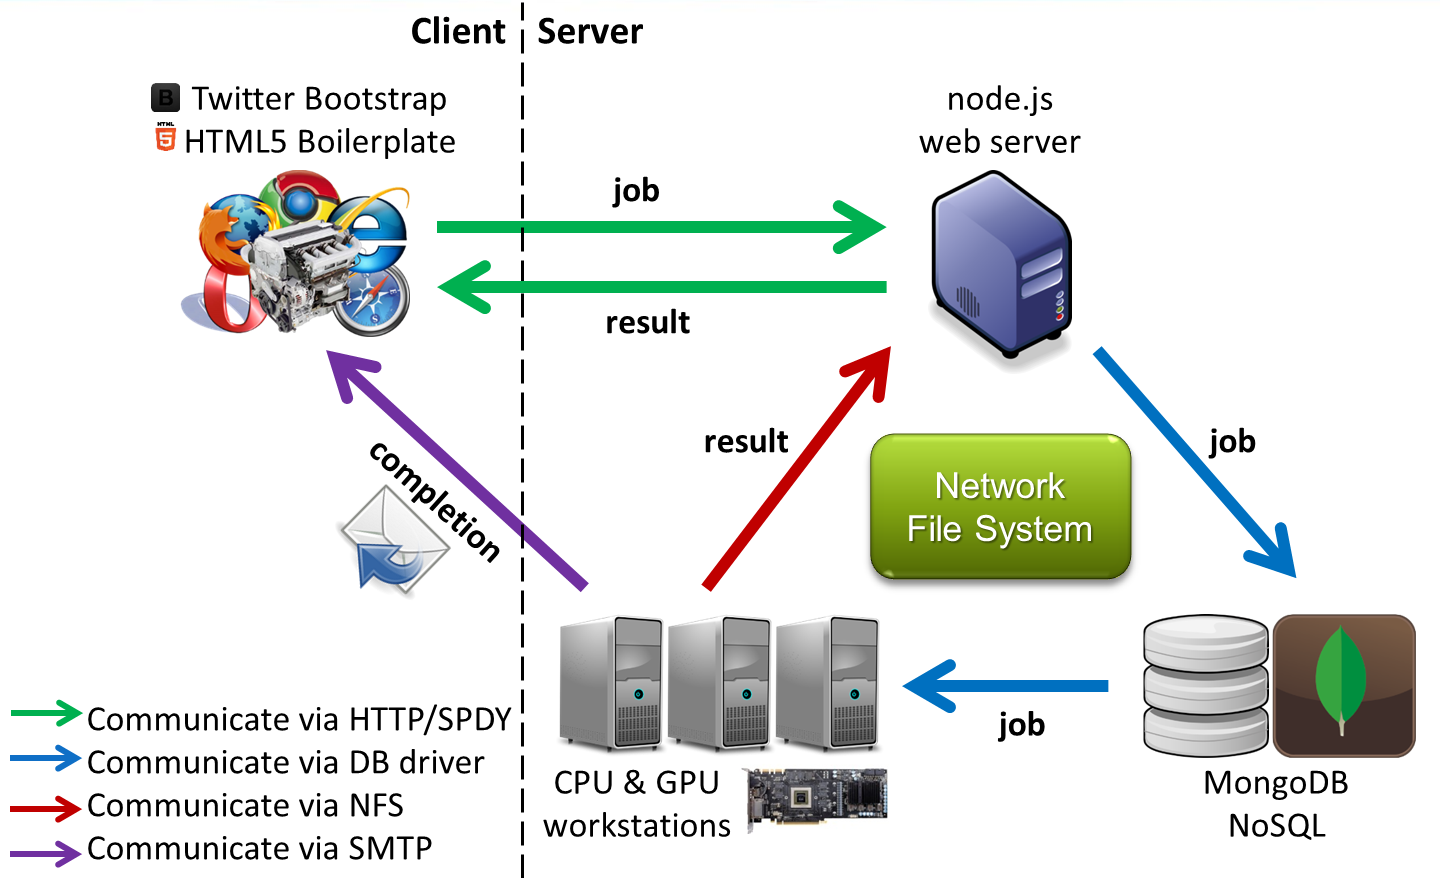
\includegraphics[width=\linewidth]{Architecture.png}}
\caption{istar architecture.}\label{istar:architecture}
\end{figure}

On the client side, we seamlessly combined both the Twitter Bootstrap and the HTML5 Boilerplate into a HTML5- and CSS3-powered web site, which was successfully checked as HTML5 by the W3C Markup Validator v1.3. We adopted the jQuery library to simplify HTML document traversing, event handling, animating, and Ajax interactions, and the jQuery UI library to provide themeable widgets. We tested our web site with Chrome 19+, Firefox 12+, Internet Explorer 9+, Safari 5+ and Opera 12+.

On the server side, we built the web server using the well-known asynchronous event-driven node.js on top of the express server, forking multiple worker processes to accept simultaneous HTTP/SPDY connections. We utilized the spdy node module to support SPDY protocol v3, the prototype of next generation HTTP 2.0, achieving reduced latency through compression, multiplexing, and prioritization. We employed the forever node module to restart worker processes automatically in case of unhandled exceptions, ensuring high availability. We made heavy use of regular expressions and developed a customized validator to validate and sanitize user input, ensuring data validity.

On the database side, we chose MongoDB, a scalable, high-performance, open source NoSQL database. MongoDB features document store in JSON style, making it particularly suitable for applications requiring flexible document attributes like our istar.

On the workstation side, we deployed a Linux workstation and four Mac workstations. The Linux workstation is equipped with Intel Xeon W3520 @ 2.66 GHz, 8GB DDR3 SDRAM and GeForce GTX 285 (1024 MB), and running Fedora 17 x64. The four Mac workstations are equipped with Intel Core i5-2400 @ 3.10GHz and 4GB DDR3 SDRAM, and running Mac OS X Lion 10.7.4.

On the network file system side, we mounted a 2TB hard disk for shared use. All the five workstations can simultaneously access to the hard disk and perform file reading and writing. In principle, we will persist existing jobs and results until storage shortage.

\section{idock on istar}

We hosted idock onto istar. On the client side, our idock web page supports filtering and previewing ligands to dock, as well as monitoring job progress in real time, two very useful and unique features. A new job consists of compulsory fields as well as optional fields. Compulsory fields include a receptor in PDBQT format, a search space defined by a cubic box, a short description of the job, and an email to receive completion notification. Optional fields include filtering conditions of ligands on 9 molecular properties (e.g. molecular weight). We set up default values for optional fields, and only the ligands satisfying all the 9 filtering conditions will be docked. We exposed job submission, job query, and ligand counting as RESTful API for others to program against. We recorded a video tutorial for newbies to get started.

On the network file system side, we collected 12,171,187 clean ligands from the ZINC database \citep{532,1178} with explicit permission. We converted all the 12 million ligands into PDBQT format, and combined them together with their 9 molecular properties into one single file as huge as 50GB for subsequent parallel docking. We recorded and encoded the offset of each ligand for fast random seeking.

On the workstation side, we developed a customized daemon of idock 1.5 in modern C++11, adding necessary code to iteratively fetch a pending job from MongoDB, reuse receptor and grid maps whenever possible, perform 2-phase docking, report progress, and send email notification upon job completion.

On one hand, our idock daemon features 2-phase docking, due to as many as 12 million ligands to screen. In phase 1, idock performs coarse but fast docking without writing any conformations, aiming to quickly shortlist a few thousand candidates. In phase 2, idock performs fine but slow docking for the candidates with a significantly larger number of Monte Carlo tasks, writing as many conformations as possible. Such a 2-phase docking methodology can remarkably reduce job execution time while avoiding the risk of filtering out potentially promising compounds.

On the other hand, our idock daemon features slice-level parallelism rather than job-level parallelism. Jobs are divided into slices, which are distributed across workstations. Slice-level parallelism is, however, much more difficult to implement. The technical hurdle becomes even more apparent when results from multiple workstations must be combined to produce a final result and progresses from multiple workstations must be combined too to compute an overall progress. Eventually we succeeded in splitting a job into 100 slices and distributing them to idle workstations in phase 1 to achieve parallel docking, better utilizing hardware.

\section{igrep on istar}

Besides idock, we hosted our igrep \citep{1138} too, a fast CUDA implementation of agrep algorithm for approximate nucleotide sequence matching. Its success demonstrates the capability of istar of hosting a general variety of programs.

\section{Discussion}

DOCK Blaster \citep{557}, an expert system, was created to investigate the feasibility of full automation of large-scale protein-ligand docking. Here we highlight the advantages of istar over DOCK Blaster. First and foremost, istar is free and open source under Apache License 2.0. Everyone is welcome to download a copy and deploy istar to his/her own servers. istar is designed as a general SaaS platform. It can host not only idock but also igrep and any other program. istar utilizes HTML5, CSS3, node.js, SPDY, NoSQL, GPU acceleration and so on, representing a state-of-the-art platform. istar supports filtering and previewing ligands to dock, as well as monitoring job progress in real time, two very useful features only available at istar. istar implements 2-phase docking and exploits fine-grained slice-level parallelism in phase 1.

Due to limited budget, we could not offer hardware resource as much as DOCK Blaster did (i.e. 700 CPU cores plus 20TB RAID-6 storage), so we tried every endeavor on software optimization. Alternatively, one can freely deploy a copy of istar. In the future we plan to port idock to GPU in order to further boost performance.

\section*{Acknowledgement}

We thank Professor John J. Irwin for granting us permission to use ZINC with three conditions as stated at istar web site.

\bibliographystyle{natbib}
\bibliography{document}

\end{document}
